\documentclass[11pt]{article}
\usepackage{amsfonts}
\usepackage{amsmath}
\usepackage{graphicx}
\usepackage{float}
\title{\textbf{CP468 Assignment 1\\Missionaries and Cannibals}}
\author{Lyndon Rey\\
		Tyler Farkas\\
		Daniel Berezovski}
\date{October 4th, 2017}

\setcounter{section}{-1}

\begin{document}

\maketitle

\section{Introduction}
\subsection{States}
For the purposes of this assignment, the following notation will be used. Firstly, any given state \(s\) will be represented by a set of two column vectors in \(\mathbb{R}^3\), both containing the elements \(m, c, b\); these elements represent the number of missionaries, number of cannibals, and whether the boat is present, respectively. Each column vector in the set represents a shoreline given in the problem: the left vector represents the starting shore, and the right vector represents the finishing shore, and the subscripts \(L\) and \(R\) represent the left and right sides, respectively. The right shore is entirely dependent on the left, as the total number of missionaries and cannibals on both shores cannot exceed the initial number, notated as \(M\) and \(C\) respectively. There is always 1 boat (\(B=1\)), so if the left shore has the boat (i.e. \(b=1)\), then the right shore will not (i.e. \(b=0)\). Thus, the abstract state can be defined as follows:
 
 \begin{equation}
s= 
\Bigg{\{}
\begin{bmatrix}
m_L\\
c_L\\
b_L
\end{bmatrix},
\begin{bmatrix}
M-m_L\\
C-c_L\\
1-b_L
\end{bmatrix}
\Bigg{\}}
\end{equation}
Continuing to formalize, the following constraints must be put on the variables:
\begin{equation}
0\leq m \leq M; \hspace{0.4cm}0 \leq c \leq C; \hspace{0.4cm} b=\{0,1\}; \hspace{0.4cm} m,c,b \in \mathbb{Z}
\end{equation}
Another restriction considered when considering possible valid states is the safety of the missionaries. Due to the cannibalistic nature of cannibals, the number of missionaries on both the left shore and right shore can never be less than the number of cannibals; i.e. \(m_L \geq c_L;\hspace{0.2cm} m_L \geq1\) and \(m_R \geq c_R;\hspace{0.2cm} m_R \geq1\) for a state to be valid.
To exemplify this, consider the state: 
 \begin{equation}
s= 
\Bigg{\{}
\begin{bmatrix}
3\\
1\\
0
\end{bmatrix},
\begin{bmatrix}
0\\
2\\
1
\end{bmatrix}
\Bigg{\}}
\hspace{0.2cm} M=3;\hspace{0.2cm} C=3; \hspace{0.2cm} B=1
\end{equation}
In this state, the left (starting) shore has all 3 missionaries, 1 cannibal, and does not have the boat. The right (finishing) shore has no missionaries (as \(m_{R} =M- m_{L}=3-3=0\)), 2 cannibals (as \(c_{R} =C- c_{L}=3-1=2\)), and the boat (as \(b_{R} =1- b_{L}=1-0=1\)). As the missionaries are never outnumbered, this is a valid state. However, if 1 missionary was moved from left to right, then the state would be invalid, as the missionaries would be outnumbered on the right shore.
\subsection{Actions}
Furthermore, all actions possible for any state will be also be represented as column vectors, with the same elements as the state column vectors (as seen in equation 1). The actions (described in section 1.2) will be of the form:
 \begin{equation}
a=
\begin{bmatrix}
m\\
c\\
b
\end{bmatrix}
\end{equation}
It must be noted that each action on any given state only directly modifies the left shore vector, as the right is dependent on the value of the left (further described in section 0.1).

\section{Problem Formulation}
\subsection{Initial State}
The initial state is simply the state in which all missionaries and cannibals, as well as the boat, are on the left shore, thus there are no people or boats on the right shore. Given in the state notation described in section 0.1:
\begin{equation}
s= 
\Bigg{\{}
\begin{bmatrix}
M\\
C\\
B
\end{bmatrix},
\begin{bmatrix}
0\\
0\\
0
\end{bmatrix}
\Bigg{\}}
\end{equation}
For example, if the maximum number of missionaries and cannibals were both 3, then the initial state would look as such:
\begin{equation}
s= 
\Bigg{\{}
\begin{bmatrix}
3\\
3\\
1
\end{bmatrix},
\begin{bmatrix}
0\\
0\\
0
\end{bmatrix}
\Bigg{\}}
\end{equation}
\subsection{Actions on States}
As stated in section 0.2, each action is represented as a column vector with the elements \(m,c,b\). The boat in question can only hold 2 people, but must hold at least 1, so \(1 \leq m+c \leq 2\). All actions require that a boat be present, so \(b=1\). An action vector can be either positive or negative, relative to the left shore: a negative action means that the boat is sailing away from the left shore, and a positive vector implies the opposite. Thus, there are 10 possible actions, with 5 negative/positive pairs. They are: 
\begin{equation}
\pm c_2=
\begin{bmatrix}
0\\
2\\
1
\end{bmatrix},
\pm c_1=
\begin{bmatrix}
0\\
1\\
1
\end{bmatrix},
\pm c_1m_1=
\begin{bmatrix}
1\\
1\\
1
\end{bmatrix},
\pm m_1=
\begin{bmatrix}
1\\
0\\
1
\end{bmatrix},
\pm m_2=
\begin{bmatrix}
2\\
0\\
1
\end{bmatrix}
\end{equation}
The notation is simply indicates how many missionaries and/or cannibals are being added or subtracted. For example, if the boat was travelling with 1 missionary and 1 cannibal from the right shore to the left shore, then this action is notated as:
\begin{equation}
+c_1m_1=\begin{bmatrix}
1\\
1\\
1
\end{bmatrix}
\end{equation}
The boat is tavelling left-to-right when \(b_L=1\), and from right-to-left when \(b_L=0\). A left-to-right action will always be negative, and a right-to-left action will always be positive (this is explained in more detail in section 1.3). 

\subsection{Transition Model}
The transition model is simple, as an action performed on a state will generate a new state by adding the left  shore vector with the action vector, and then calculating the right shore vector using the generated left shore vector. Formalized:
\begin{equation}
\text{Result}(s,a) = \vec{s_L}+\vec{a}
\end{equation}
This equation only holds true when \(\text{Result}(s,a)\) is a valid state, using all the guidelines given in section 0.1. For example, if:
\begin{equation}
s= 
\Bigg{\{}
\begin{bmatrix}
3\\
3\\
1
\end{bmatrix},
\begin{bmatrix}
0\\
0\\
0
\end{bmatrix}
\Bigg{\}}
\text{ and } a=-c_1=-
\begin{bmatrix}
0\\
1\\
1\\
\end{bmatrix}
\end{equation} 
then:
\begin{equation}
\text{Result}(s,a)=\vec{s_L}+\vec{a}=
\begin{bmatrix}
3\\3\\1
\end{bmatrix}
-
\begin{bmatrix}
0\\1\\1
\end{bmatrix}
=
\begin{bmatrix}
3\\2\\0
\end{bmatrix}
\end{equation}
so the generated state would be:
\begin{equation}
s= 
\Bigg{\{}
\begin{bmatrix}
3\\
2\\
0
\end{bmatrix},
\begin{bmatrix}
0\\
1\\
1
\end{bmatrix}
\Bigg{\}}
\end{equation}
which is a valid state, given the terms in section 0.1. This means that the boat brought 1 cannibal from the left shore to the right shore.

\subsection{Goal Test}
The goal test is to check whether the left shore is empty in a given state. Formally, the goal is achieved when:
\begin{equation}
s= 
\Bigg{\{}
\begin{bmatrix}
0\\
0\\
0
\end{bmatrix},
\begin{bmatrix}
3\\
3\\
1
\end{bmatrix}
\Bigg{\}}
\end{equation}
From this, a Boolean function can be created:
\begin{equation}
\text{Goal}(s) = \begin{cases} \text{True,} & \text{if } s_L=\vec{0} \\ \text{False,} & \text{if } s_L\neq\vec{0} \end{cases}
\end{equation}

\subsection{Path Cost}
The cost of each boat trip across the river is 1, so the path cost is the number of river crossings. The optimal path is the path in which the boat crosses the river the fewest times. 

\section{State Space Diagram}
In the following state space diagram, it is assumed that each river crossing alternates addition and subraction, beginning with subtraction. However, each action is bidirectional, and if going from a frontier state back to a previously-seen state, then the sign of the action is reversed (this should never happen, as looping paths will never be more optimal than non-looping paths).
\begin{figure}[H] 
  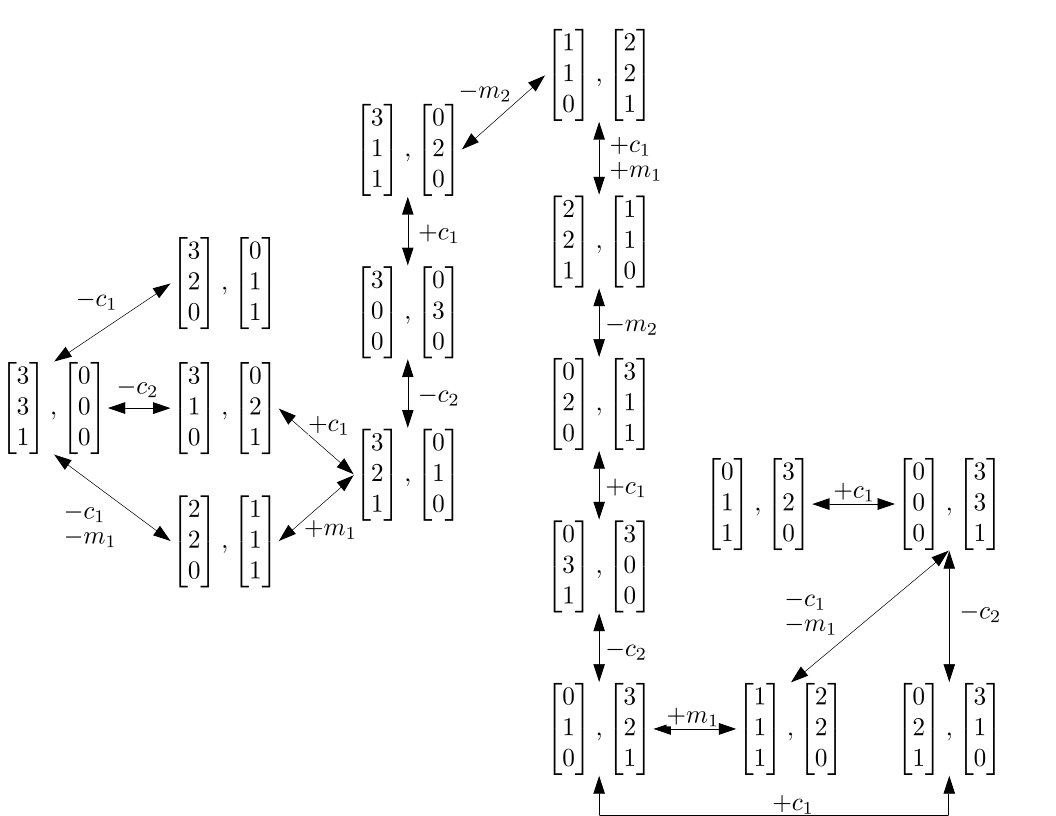
\includegraphics[scale=0.5]{State-Space-Matrices.png}
\end{figure}

\section{Implementation}
\end{document}
